\begin{figure}
    \resizebox{.5\linewidth}{!}{
        \subfloat[Average Latency vs. Area]{
            file encoding: UTF-8
=========================================================
Please add the following lines to your LaTeX preamble:

\usepackage[utf8]{inputenc}
\usepackage{fontspec}
\usepackage{pgfplots}
\usepgfplotslibrary{plotmarks}
=========================================================
% This file was created by matplotlib2tikz v0.5.15.
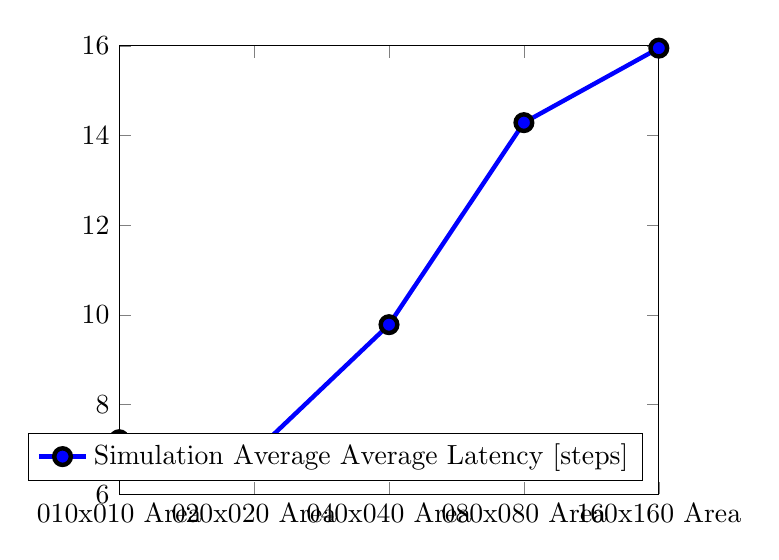
\begin{tikzpicture}

\begin{axis}[
xmin=0, xmax=4,
ymin=6, ymax=16,
axis on top,
xtick={0,1,2,3,4},
xticklabels={010x010 Area,020x020 Area,040x040 Area,080x080 Area,160x160 Area},
legend entries={{Simulation Average Average Latency [steps]}},
legend style={at={(0.97,0.03)}, anchor=south east},
legend cell align={left}
]
\addplot [ultra thick, blue, mark=*, mark size=3, mark options={solid,draw=black}]
table {%
0 7.214
1 6.918
2 9.78
3 14.286
4 15.948
};
\end{axis}

\end{tikzpicture}

        }
    }
    \resizebox{.5\linewidth}{!}{
        \subfloat[Success Rate vs. Area]{
            file encoding: UTF-8
=========================================================
Please add the following lines to your LaTeX preamble:

\usepackage[utf8]{inputenc}
\usepackage{fontspec}
\usepackage{pgfplots}
\usepgfplotslibrary{plotmarks}
=========================================================
% This file was created by matplotlib2tikz v0.5.15.
\begin{tikzpicture}

\begin{axis}[
xmin=0, xmax=4,
ymin=10, ymax=100,
axis on top,
xtick={0,1,2,3,4},
xticklabels={010x010 Area,020x020 Area,040x040 Area,080x080 Area,160x160 Area},
legend entries={{Simulation Average Success Rate [%]}},
legend cell align={left},
legend style={at={(0.97,0.03)}, anchor=south east}
]
\addplot [ultra thick, blue, mark=*, mark size=3, mark options={solid,draw=black}]
table {%
0 100
1 83.86
2 62.81
3 38.908
4 16.802
};
\end{axis}

\end{tikzpicture}

        }
    }
    \caption{Network Properties with Increasing Area given Constant Radius and Number of Users}
    \label{fig:vararea}
\end{figure}
Linear increase Latency, linear decrease in success rate (increase in dropped packets)

\begin{figure}
    \resizebox{.5\linewidth}{!}{
        \subfloat[Average Latency vs. Radius]{
            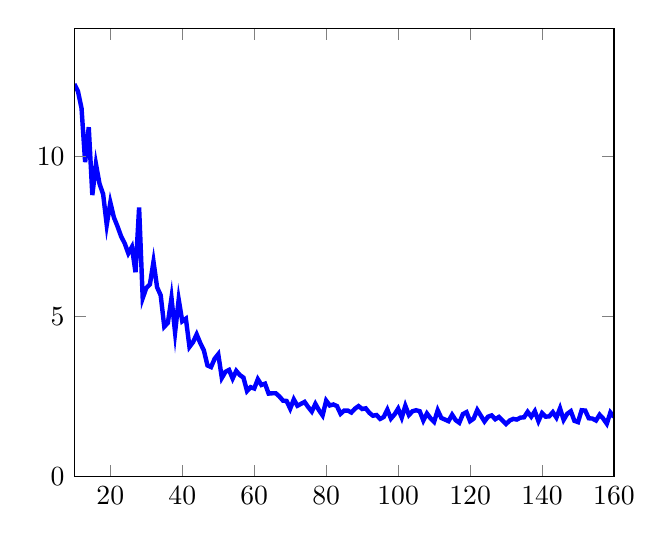
\begin{tikzpicture}

\begin{axis}[
xmin=10, xmax=160,
ymin=0, ymax=14,
axis on top
]
\addplot [ultra thick, blue]
table {%
10 12.26
11 12.03
12 11.5
13 9.82
14 10.91
15 8.79
16 9.76
17 9.14
18 8.82
19 7.86
20 8.56
21 8.09
22 7.81
23 7.5
24 7.28
25 6.97
26 7.17
27 6.38
28 8.4
29 5.57
30 5.89
31 6
32 6.71
33 5.91
34 5.66
35 4.68
36 4.8
37 5.58
38 4.5
39 5.53
40 4.85
41 4.93
42 4.05
43 4.2
44 4.44
45 4.17
46 3.94
47 3.47
48 3.42
49 3.68
50 3.82
51 3.08
52 3.27
53 3.33
54 3.06
55 3.3
56 3.17
57 3.09
58 2.67
59 2.79
60 2.75
61 3.04
62 2.86
63 2.9
64 2.59
65 2.6
66 2.6
67 2.5
68 2.37
69 2.36
70 2.12
71 2.41
72 2.21
73 2.27
74 2.33
75 2.17
76 2.03
77 2.27
78 2.07
79 1.91
80 2.37
81 2.22
82 2.25
83 2.2
84 1.96
85 2.06
86 2.06
87 2
88 2.12
89 2.2
90 2.11
91 2.13
92 1.99
93 1.9
94 1.92
95 1.8
96 1.86
97 2.09
98 1.81
99 1.94
100 2.12
101 1.84
102 2.21
103 1.92
104 2.04
105 2.07
106 2.04
107 1.75
108 1.97
109 1.82
110 1.71
111 2.07
112 1.83
113 1.78
114 1.73
115 1.93
116 1.76
117 1.68
118 1.95
119 2.01
120 1.73
121 1.81
122 2.08
123 1.9
124 1.72
125 1.87
126 1.91
127 1.79
128 1.86
129 1.75
130 1.64
131 1.75
132 1.8
133 1.78
134 1.84
135 1.85
136 2.02
137 1.87
138 2.04
139 1.73
140 1.98
141 1.87
142 1.88
143 2.01
144 1.84
145 2.13
146 1.77
147 1.96
148 2.04
149 1.74
150 1.7
151 2.07
152 2.06
153 1.82
154 1.81
155 1.75
156 1.93
157 1.81
158 1.65
159 2
160 1.86
};
\end{axis}

\end{tikzpicture}

        }
    }
    \resizebox{.5\linewidth}{!}{
        \subfloat[Success Rate vs. Radius]{
            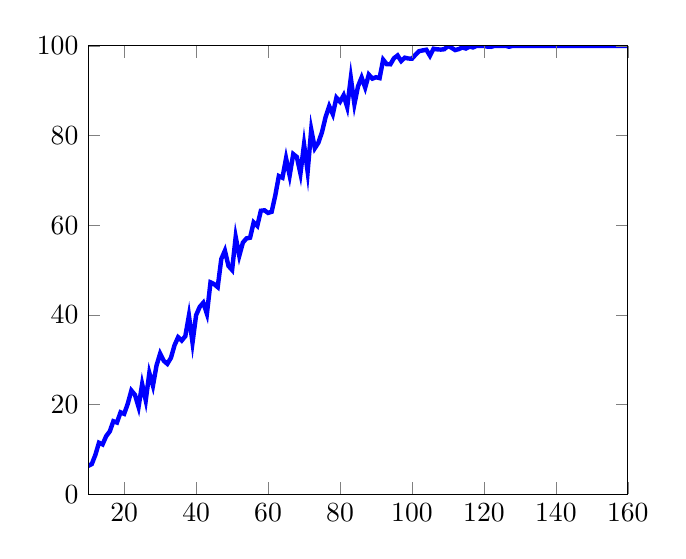
\begin{tikzpicture}

\begin{axis}[
xmin=10, xmax=160,
ymin=0, ymax=100,
axis on top
]
\addplot [ultra thick, blue]
table {%
10 6.29
11 6.71
12 8.76
13 11.47
14 11.09
15 12.93
16 13.99
17 16.26
18 15.97
19 18.25
20 17.91
21 20.16
22 23.11
23 22.15
24 19.45
25 24.54
26 20.92
27 27.03
28 24.19
29 28.7
30 31.35
31 29.75
32 29.06
33 30.39
34 33.2
35 35
36 34.26
37 35.24
38 39.81
39 33.81
40 39.92
41 41.76
42 42.69
43 40.23
44 47.24
45 46.85
46 46.18
47 52.45
48 54.3
49 50.89
50 50
51 57.36
52 53.17
53 56.11
54 57.04
55 57.2
56 60.61
57 59.84
58 63.21
59 63.31
60 62.73
61 62.98
62 66.6
63 70.95
64 70.58
65 74.9
66 71.07
67 75.85
68 75.2
69 71.51
70 78.01
71 71.93
72 81.31
73 77.16
74 78.4
75 80.79
76 84.13
77 86.53
78 84.75
79 88.43
80 87.53
81 88.96
82 86.33
83 92.83
84 87
85 90.95
86 92.94
87 90.68
88 93.57
89 92.68
90 92.99
91 92.8
92 96.9
93 95.9
94 95.88
95 97.24
96 97.85
97 96.6
98 97.35
99 97.17
100 97.13
101 98.02
102 98.8
103 98.98
104 99.12
105 97.78
106 99.35
107 99.21
108 99.16
109 99.24
110 100
111 99.57
112 99.05
113 99.26
114 99.64
115 99.39
116 99.81
117 99.64
118 100
119 100
120 100
121 99.81
122 99.78
123 100
124 100
125 100
126 100
127 99.8
128 100
129 100
130 100
131 100
132 100
133 100
134 100
135 100
136 100
137 100
138 100
139 100
140 100
141 100
142 100
143 100
144 100
145 100
146 100
147 100
148 100
149 100
150 100
151 100
152 100
153 100
154 100
155 100
156 100
157 100
158 100
159 100
160 100
};
\end{axis}

\end{tikzpicture}

        }
    }
    \caption{Network Properties with Increasing Radius Area given Constant Area and Number of Users}
    \label{fig:varradius}
\end{figure}
Non-linear decrease in latency, non-linear increase in success rate

\begin{figure}
    \resizebox{.5\linewidth}{!}{
        \subfloat[Average Latency vs. Number of Users]{
            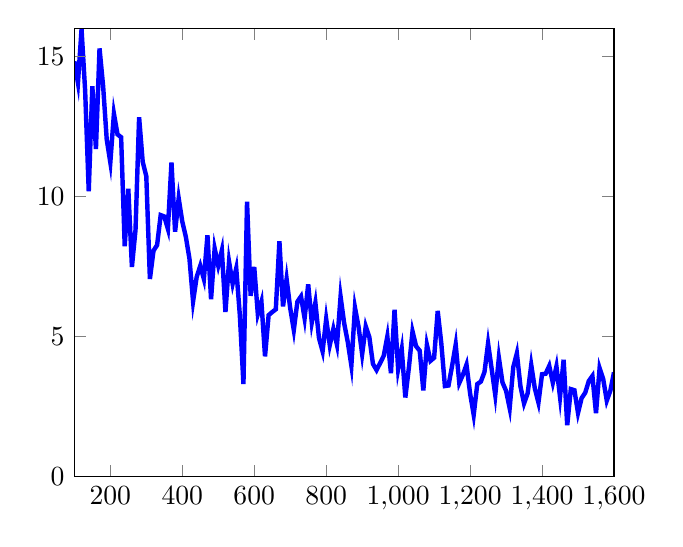
\begin{tikzpicture}

\begin{axis}[
xmin=100, xmax=1600,
ymin=0, ymax=16,
axis on top
]
\addplot [ultra thick, blue]
table {%
100 14.82
110 14.05
120 15.96
130 13.77
140 10.18
150 13.93
160 11.69
170 15.28
180 13.93
190 12.03
200 11.21
210 12.95
220 12.21
230 12.11
240 8.22
250 10.27
260 7.48
270 8.8
280 12.82
290 11.23
300 10.72
310 7.05
320 8.06
330 8.26
340 9.33
350 9.28
360 8.84
370 11.21
380 8.74
390 9.93
400 9.1
410 8.55
420 7.77
430 6.25
440 7.12
450 7.52
460 7.05
470 8.61
480 6.33
490 8.14
500 7.53
510 8.07
520 5.87
530 7.67
540 6.88
550 7.43
560 5.76
570 3.3
580 9.81
590 6.45
600 7.48
610 5.8
620 6.24
630 4.29
640 5.76
650 5.87
660 5.97
670 8.4
680 6.07
690 7.05
700 6.01
710 5.23
720 6.24
730 6.43
740 5.65
750 6.86
760 5.5
770 6.2
780 4.94
790 4.47
800 5.62
810 4.69
820 5.27
830 4.7
840 6.42
850 5.47
860 4.8
870 3.96
880 6.03
890 5.34
900 4.37
910 5.36
920 4.97
930 4.02
940 3.8
950 4.05
960 4.31
970 5
980 3.69
990 5.95
1000 3.84
1010 4.54
1020 2.82
1030 3.9
1040 5.18
1050 4.65
1060 4.49
1070 3.07
1080 4.7
1090 4.13
1100 4.24
1110 5.91
1120 4.75
1130 3.23
1140 3.25
1150 3.95
1160 4.71
1170 3.34
1180 3.63
1190 3.99
1200 2.97
1210 2.2
1220 3.3
1230 3.39
1240 3.73
1250 4.75
1260 3.84
1270 2.91
1280 4.24
1290 3.36
1300 3.06
1310 2.44
1320 3.9
1330 4.4
1340 3.22
1350 2.61
1360 2.97
1370 3.98
1380 3.14
1390 2.64
1400 3.65
1410 3.67
1420 3.95
1430 3.35
1440 3.93
1450 2.84
1460 4.17
1470 1.83
1480 3.12
1490 3.08
1500 2.27
1510 2.8
1520 2.99
1530 3.41
1540 3.59
1550 2.26
1560 3.87
1570 3.48
1580 2.71
1590 3.07
1600 3.72
};
\end{axis}

\end{tikzpicture}

        }
    }
    \resizebox{.5\linewidth}{!}{
        \subfloat[Sucess Rate vs. Number of Users]{
            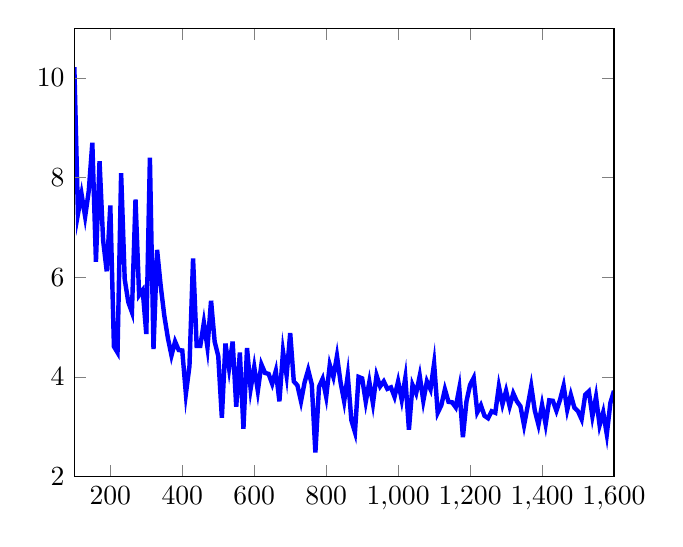
\begin{tikzpicture}

\begin{axis}[
xmin=100, xmax=1600,
ymin=2, ymax=11,
axis on top
]
\addplot [ultra thick, blue]
table {%
100 10.22
110 7.27
120 7.67
130 7.22
140 7.73
150 8.7
160 6.31
170 8.33
180 6.74
190 6.12
200 7.44
210 4.61
220 4.49
230 8.09
240 5.96
250 5.5
260 5.3
270 7.56
280 5.64
290 5.74
300 4.86
310 8.4
320 4.56
330 6.55
340 5.83
350 5.23
360 4.78
370 4.43
380 4.71
390 4.54
400 4.53
410 3.66
420 4.22
430 6.38
440 4.62
450 4.62
460 5.09
470 4.59
480 5.53
490 4.71
500 4.42
510 3.18
520 4.67
530 4.17
540 4.71
550 3.4
560 4.49
570 2.96
580 4.58
590 3.76
600 4.2
610 3.72
620 4.25
630 4.08
640 4.06
650 3.86
660 4.12
670 3.51
680 4.51
690 4.03
700 4.88
710 3.91
720 3.83
730 3.51
740 3.89
750 4.14
760 3.85
770 2.48
780 3.8
790 3.96
800 3.6
810 4.24
820 4
830 4.42
840 3.89
850 3.51
860 4.03
870 3.13
880 2.89
890 4
900 3.97
910 3.5
920 3.9
930 3.47
940 4.03
950 3.81
960 3.91
970 3.76
980 3.79
990 3.6
1000 3.91
1010 3.54
1020 3.98
1030 2.94
1040 3.84
1050 3.67
1060 4.02
1070 3.52
1080 3.91
1090 3.75
1100 4.27
1110 3.28
1120 3.43
1130 3.75
1140 3.5
1150 3.49
1160 3.39
1170 3.77
1180 2.79
1190 3.51
1200 3.84
1210 3.98
1220 3.29
1230 3.43
1240 3.22
1250 3.17
1260 3.31
1270 3.28
1280 3.81
1290 3.45
1300 3.72
1310 3.41
1320 3.67
1330 3.51
1340 3.41
1350 3.03
1360 3.41
1370 3.81
1380 3.32
1390 3.04
1400 3.44
1410 3.05
1420 3.53
1430 3.52
1440 3.32
1450 3.54
1460 3.82
1470 3.34
1480 3.64
1490 3.38
1500 3.31
1510 3.15
1520 3.64
1530 3.71
1540 3.21
1550 3.6
1560 3.03
1570 3.29
1580 2.85
1590 3.48
1600 3.72
};
\end{axis}

\end{tikzpicture}

        }
    }
    \caption{Network Properties with Increasing Number of Users given Constant Area and Radius}
    \label{fig:varusers}
\end{figure}
Linear Reudction in latency, Non-linear reduction in success rate
